	% ---------------------------------------------------------------------------
% ---------------------------------------------------------------------------
% Modelo LaTex para preparação do documento final de Dissertação de Mestrado
% O modelo está em conformidade com ABNT NBR 14724:2011: 
% Programa de Pós-Graduação em Informática
% Universidade Federal de Alagoas
% Versão: v0.9
% ---------------------------------------------------------------------------
% ---------------------------------------------------------------------------

\documentclass[
	% -- opções da classe memoir --
	12pt,					% tamanho da fonte
	openright,				% capítulos começam em pág ímpar (insere página vazia caso preciso)
	twoside,					% para impressão em verso e anverso. Oposto a oneside
	a4paper,					% tamanho do papel. 
	% -- opções da classe abntex2 --
	chapter=TITLE,			% títulos de capítulos convertidos em letras maiúsculas
	%section=TITLE,			% títulos de seções convertidos em letras maiúsculas
	%subsection=TITLE,		% títulos de subseções convertidos em letras maiúsculas
	%subsubsection=TITLE,	% títulos de subsubseções convertidos em letras maiúsculas
	% -- opções do pacote babel --
	english,				% idioma adicional para hifenização
	%french,				% idioma adicional para hifenização
	%spanish,				% idioma adicional para hifenização
	brazil					% o último idioma é o principal do documento
]{abntex2}

% ---------------------
% Pacotes OBRIGATÓRIOS
% ---------------------
\usepackage[T1]{fontenc}			% Selecao de codigos de fonte.
\usepackage[utf8]{inputenc}		% Codificacao do documento (conversão automática dos acentos)
\usepackage{lastpage}				% Usado pela Ficha catalográfica
\usepackage{indentfirst}				% Indenta o primeiro parágrafo de cada seção.
\usepackage{color}						% Controle das cores
\usepackage{graphicx,graphicx}	% Inclusão de gráficos
\usepackage{epsfig,subfig}			% Inclusão de figuras
\usepackage{microtype} 				% Melhorias de justificação
% ---------------------
		
% ---------------------
% Pacotes ADICIONAIS
% ---------------------
\usepackage{lipsum}									% Geração de dummy text
\usepackage{amsmath,amssymb,mathrsfs}	% Comandos matemáticos avançados 
\usepackage{setspace}  								% Para permitir espaçamento simples, 1 1/2 e duplo
\usepackage{verbatim}								% Para poder usar o ambiente "comment"
\usepackage{tabularx} 								% Para poder ter tabelas com colunas de largura auto-ajustável
\usepackage{afterpage} 								% Para executar um comando depois do fim da página corrente
\usepackage{url} 										% Para formatar URLs (endereços da Web)
\usepackage{enumitem}
\usepackage{svg}
% ---------------------

% ---------------------
% Pacotes de CITAÇÕES
% ---------------------
\usepackage[brazilian,hyperpageref]{backref}	% Paginas com as citações na bibl
\usepackage[alf]{abntex2cite}				% Citações padrão ABNT (alfa)
%\usepackage[num]{abntex2cite}				% Citações padrão ABNT (numericas)
% ---------------------

% Definição de diretório de imagens
\graphicspath{{imagens/}}

% Configurações de CITAÇÕES para abntex2
% --- 
% CONFIGURAÇÕES DE PACOTES
% --- 

% ---
% Configurações do pacote backref
% Usado sem a opção hyperpageref de backref
%\renewcommand{\backrefpagesname}{Citado na(s) página(s):~}
% Texto padrão antes do número das páginas
%\renewcommand{\backref}{}
% Define os textos da citação
%\renewcommand*{\backrefalt}[4]{
%	\ifcase #1 %
%		Nenhuma citação no texto.%
%	\or
%		Citado na página #2.%
%	\else
%		Citado #1 vezes nas páginas #2.%
%	\fi}%
% ---

% Inclusão de dados para CAPA e FOLHA DE ROSTO (título, autor, orientador, etc.)
% ---
% Informações de dados para CAPA e FOLHA DE ROSTO
% ---
\titulo{UMA ABORDAGEM EM CASCATA PARA O ALINHAMENTO DE DADOS CONECTADOS}
\autor{Armando Barbosa Sobrinho}
\local{Maceió-AL}
\data{2016}
\orientador{Ig Ibert Bittencourt Santana Pinto}
\coorientador{Sean Wolfgand Matsui Siqueira}
\instituicao{%
  Universidade Federal de Alagoas -- UFAL
  \par
  Instituto de Computação
  \par
  Programa de Pós-Graduação em Informática
}
\tipotrabalho{Dissertação (Mestrado)}
% O preambulo deve conter o tipo do trabalho, o objetivo,
% o nome da instituição e a área de concentração
\preambulo{Dissertação apresentada como requisito parcial para obtenção do grau de Mestre pelo Programa de Pós-Graduação em Informática do Instituto de Computação da Universidade Federal de Alagoas.}
% ---

% Inclui Configurações de aparência do PDF Final
%  Configurações de aparência do PDF final
% NÃO ALTERAR!!!

% alterando o aspecto da cor azul
\definecolor{blue}{RGB}{41,5,195}

% informações do PDF
\makeatletter
\hypersetup{
     	%pagebackref=true,
		pdftitle={\@title}, 
		pdfauthor={\@author},
    		pdfsubject={\imprimirpreambulo},
	    pdfcreator={LaTeX with abnTeX2},
		pdfkeywords={abnt}{latex}{abntex}{abntex2}{trabalho acadêmico}, 
		colorlinks=true,       		% false: boxed links; true: colored links
    		linkcolor=black,          	% color of internal links
    		citecolor=black,        		% color of links to bibliography
    		filecolor=black,      		% color of file links
		urlcolor=black,
		bookmarksdepth=4
} 
\makeatother
% --- 

% Inclui configurações da folha de rosto
\renewcommand{\folhaderostocontent}{
	\begin{center}
		\MakeUppercase{\imprimirautor}
		
		\vspace*{\fill}
		\vspace*{\fill}
		\textbf{\imprimirtitulo}
		
		\vspace*{\fill}
		\hspace{.45\textwidth}
		\begin{minipage}{.5\textwidth}
			\SingleSpacing
			\imprimirpreambulo
			
			\vspace*{1cm}
			\imprimirorientadorRotulo~\imprimirorientador
			\par
			\imprimircoorientadorRotulo~\imprimircoorientador
		\end{minipage}
		
		\vspace*{\fill}
		\vspace*{\fill}
		\imprimirlocal
		\par
		\imprimirdata
	\end{center}
}


% Configurações da fonte do texto
\usepackage{times}						% Usar a fonte Times New Roman
\renewcommand{\ABNTEXpartfontsize}{\normalsize}
\renewcommand{\ABNTEXsectionfontsize}{\normalsize}
\renewcommand{\ABNTEXsubsectionfontsize}{\normalsize}
\renewcommand{\ABNTEXsubsubsectionfontsize}{\normalsize}
\renewcommand{\ABNTEXsubsubsubsectionfontsize}{\normalsize}
\renewcommand{\ABNTEXchapterfontsize}{\normalsize}

%\chapterstyle{article}
\renewcommand{\ABNTEXchapterfont}{\fontseries{b}}

% O tamanho da identação do parágrafo é dado por:
\setlength{\parindent}{1.3cm}

% Controle do espaçamento entre um parágrafo e outro:
\setlength{\parskip}{0.2cm}  % tente também \onelineskip

% Espaço entre o título do capítulo e o texto
\setlength{\afterchapskip}{0.8cm}

% ---------------------
% Compila o indice
% ---------------------
\makeindex
% ---------------------

%%%%%%%%%%%%%%%%%%%%%%%%%%%
%%  INICIO DO DOCUMENTO  %%
%%%%%%%%%%%%%%%%%%%%%%%%%%%
\begin{document}

% Elementos textuais com numeração arábica
\pagenumbering{arabic}

% Retira espaço extra obsoleto entre as frases.
\frenchspacing

% ----------------------------------------------------------
% ELEMENTOS PRÉ-TEXTUAIS (Capa, Resumo, Abstract, etc.)
% ----------------------------------------------------------
\pretextual

% Capa
% ---
% Impressão da Capa
% ---
\begin{capa}
	\center
	UNIVERSIDADE FEDERAL DE ALAGOAS\\
	INSTITUTO DE COMPUTAÇÃO\\
	PROGRAMA DE PÓS GRADUAÇÃO EM INFORMÁTICA

	\vfill
	\MakeUppercase{\imprimirautor}

    \vfill
    \textbf{\imprimirtitulo}
    \vfill
    
    \vfill
    \imprimirlocal
    \par
    \imprimirdata

    \vspace*{1cm}
\end{capa}
% ---

% Folha de rosto (o * indica que haverá a ficha bibliográfica)
\imprimirfolhaderosto

% Imprimir Ficha Catalografica
%% ---
% Ficha Catalográfica
% ---
% Isto é um exemplo de Ficha Catalográfica, ou ``Dados internacionais de
% catalogação-na-publicação''. Você pode utilizar este modelo como referência. 
% Porém, provavelmente a biblioteca da sua universidade lhe fornecerá um PDF
% com a ficha catalográfica definitiva após a defesa do trabalho. Quando estiver
% com o documento, salve-o como PDF no diretório do seu projeto e substitua todo
% o conteúdo de implementação deste arquivo pelo comando abaixo:
%
% \begin{fichacatalografica}
%     \includepdf{fig_ficha_catalografica.pdf}
% \end{fichacatalografica}
\begin{fichacatalografica}
	\vspace*{\fill}					% Posição vertical
	\hrule							% Linha horizontal
	\begin{center}					% Minipage Centralizado
	\begin{minipage}[c]{12.5cm}		% Largura
	
	\imprimirautor
	
	\hspace{0.5cm} \imprimirtitulo  / \imprimirautor. --
	\imprimirlocal, \imprimirdata-
	
	\hspace{0.5cm} \pageref{LastPage} p. : il. (algumas color.) ; 30 cm.\\
	
	\hspace{0.5cm} \imprimirorientadorRotulo~\imprimirorientador\\
	
	\hspace{0.5cm}
	\parbox[t]{\textwidth}{\imprimirtipotrabalho~--~\imprimirinstituicao,
	\imprimirdata.}\\
	
	\hspace{0.5cm}
		1. Palavra-chave1.
		2. Palavra-chave2.
		I. Orientador.
		II. Universidade xxx.
		III. Faculdade de xxx.
		IV. Título\\ 			
	
	\hspace{8.75cm} CDU 02:141:005.7\\
	
	\end{minipage}
	\end{center}
	\hrule
\end{fichacatalografica}
% ---

% Inserir Folha de Aprovação
%% ---
% Assinaturas
% ---
% Isto é um exemplo de Folha de aprovação, elemento obrigatório da NBR
% 14724/2011 (seção 4.2.1.3). Você pode utilizar este modelo até a aprovação
% do trabalho. Após isso, substitua todo o conteúdo deste arquivo por uma
% imagem da página assinada pela banca com o comando abaixo:
%
% \includepdf{folhadeaprovacao_final.pdf}
%
\begin{folhadeaprovacao}
	\begin{center}
		\textbf{Folha de Aprovação}
		\vfill
		
		AUTOR: \MakeUppercase{\imprimirautor}
				
		\vfill
		\imprimirtitulo
		\vfill
		
		\hspace{.45\textwidth}
		\begin{minipage}{.5\textwidth}
			\imprimirpreambulo
		\end{minipage}%
		\vfill
	    
		Trabalho aprovado. \imprimirlocal, 28 de setembro de 2016:
	\end{center}
	
	\assinatura{\textbf{\imprimirorientador} \\ Orientador} 
	\assinatura{\textbf{\imprimircoorientador} \\ Co-Orientador} 
	\assinatura{\textbf{Professor} \\ Convidado 1}
	\assinatura{\textbf{Professor} \\ Convidado 2}
	
\end{folhadeaprovacao}

% Dedicatória
%% ---
% Dedicatória
% ---
\begin{dedicatoria}
   \vspace*{\fill}
   \centering
   \noindent
   \textit{ À Deus, pois sem sua força não conseguiria superar meus obstáculos. \\
   Aos meus pais Joana e Ednaldo, \\ 
   			por sempre estarem comigo em todos os 				momentos.} \vspace*{\fill}
\end{dedicatoria}
% ---

% Agradecimentos
%% ---
% Agradecimentos
% ---
\begin{agradecimentos}

Agradeço a Deus.

Agradeço aos meus pais, XXXXX e YYYYY, por ...

Aos meus irmãos, por.....

Agradeço ao meu orientador, XXXXXXXXX, por todos os conselhos, pela paciência e ajuda nesse período.

Aos meus amigos ...

Aos professores ...

À XXXXXX pelo apoio financeiro para realização deste trabalho de pesquisa.

\end{agradecimentos}
%% ---

% Epígrafe
%% ---
% Epígrafe
% ---
\begin{epigrafe}
    \vspace*{\fill}
	\begin{flushright}
		\textit{``Eu acredito demais na sorte.\\ 					E tenho constatado que, \\
        		quanto mais duro eu trabalho,\\ 				mais sorte eu tenho.''\\
		          (Thomas Jefferson)}
	\end{flushright}
\end{epigrafe}
% ---

% Resumo e Abstract
% ---
% RESUMOS
% ---

% RESUMO em português
\setlength{\absparsep}{18pt} % ajusta o espaçamento dos parágrafos do resumo
\begin{resumo}
Atualmente várias iniciativas de abertura de dados vêm sendo realizadas ao redor do mundo, dessas iniciativas a maior parte é provida pelo segmento governamental através da publicação de seus dados. permitindo que governo e sociedade civil faça uso das informações das mais diversas formas. Por Exemplo, no desenvolvimento de aplicações para melhorar a tomada de decisão por parte do governo, bem como, em aplicações que possam ser utilizadas diretamente pela sociedade. 

Apesar dos benefícios providos pela crescente oferta de dados, é possível ressaltar problemas que ainda estão em aberto, como, por exemplo, o baixo reuso dos dados publicados, baixa integração e não utilização de padrões para a descrição desses dados, acarretando em uma baixa interoperabilidade. Baseando-se nessas questões, abordagens que objetivem integrar dados ou que permitiam uma maior interoperabilidade  merecem destaque. Dessa forma, Dados Conectados se torna uma alternativa considerável para a resolução de tais questões.

Um problema existente na comunidade de Dados Conectados relacionado à integração de informação entre diferentes \textit{datasets} é chamado de problema de correspondência de instâncias do inglês (\textit{Instance Matching}), que se trata de encontrar instâncias em \textit{datasets} diferentes que se referem a mesma entidade do mundo real. Neste contexto, este trabalho propõe uma abordagem para a correspondência de instâncias.

 \textbf{Palavras-chaves}: Correspondência de Instâncias, Alinhamento de Dados, \textit{Datasets}, Dados Conectados, Web de Dados.
\end{resumo}

% ABSTRACT in english
\begin{resumo}[Abstract]
 \begin{otherlanguage*}{english}
   TODO.

   \vspace{\onelineskip}
 
   \noindent 
   \textbf{Keywords}: TODO.
 \end{otherlanguage*}
\end{resumo}

% Lista de ilustrações
\pdfbookmark[0]{\listfigurename}{lof}
\listoffigures*
\cleardoublepage

% Lista de tabelas
\pdfbookmark[0]{\listtablename}{lot}
\listoftables*
\cleardoublepage

% Lista de abreviaturas e siglas
%\begin{siglas}
%  \item[ABNT] Associação Brasileira de Normas Técnicas
%  \item[abnTeX] ABsurdas Normas para TeX
%\end{siglas}

% Lista de símbolos
%\begin{simbolos}
%  \item[$ \Gamma $] Letra grega Gama
%  \item[$ \Lambda $] Lambda
%  \item[$ \zeta $] Letra grega minúscula zeta
%  \item[$ \in $] Pertence
%\end{simbolos}

% Inserir o SUMÁRIO
\pdfbookmark[0]{\contentsname}{toc}
\tableofcontents*
\cleardoublepage

% ----------------------------------------------------------
% ELEMENTOS TEXTUAIS (Capítulos)
% ----------------------------------------------------------
\textual

% Ajusta o header para conter apenas o número da página
\pagestyle{simple}

% ----------------------------------------------------------
% TEXTO DA DISSERTAÇÃO
% ----------------------------------------------------------
\chapter{Introdução}
\label{cap:introducao}
O Atual paradigma da Web é descrito como Web de documentos. Neste, os documentos ou páginas são descritas através de uma linguagem de marcação de hipertexto (HTML) e interligados através de hiperlinks. Para identificar as páginas na Web, é necessário um mecanismo capaz de identificar de forma única cada uma dessas páginas. Para isso, a identificação é realizada através de um mecanismo de identificação global chamado URI (Uniform Resource Identifier). Dessa forma, para ter acesso a um conteúdo específico de qualquer documento neste paradigma, é necessário obter todo o documento.

Diferentemente da Web de documentos, a Web de dados, através de URIs, possibilita que os dados sejam identificados de forma única, permitindo que apenas os dados desejados sejam recuperados.  Consequentemente, essas páginas assumem um papel de conjunto de dados (datasets). Além disso, os dados são representados através de um framework de descrição de recursos (RDF) e uma linguagem de consulta aos dados, linguagem SPARQL. Através desses recursos, é possível apontar e navegar entre os dados na Web. Surgindo o conceito de Dados Conectados.

O conceito de Dados Conectados está intimamente relacionado à Web de dados, pois de acordo com \citeonline{bizer2009linked}, Dados Conectados trata-se de usar a Web para criar links entre dados de fontes diferentes. Além disso, Dados Conectados é considerado um ponto chave para o desenvolvimento da Web Semântica \cite{berners2001semantic} . Além disso, \citeonline{Isotani2015} destacam seu potencial de aplicação, tando para negócios quanto para o governo.  
Caso como o da BestBuy, que través da utilização de serialização RDF (RDFa) melhorou o número de acessos via buscador  Google entre 15\% e 30\%. Além do próprio Google, que passou a utilizar a serialização json-ld em um de seus produtos, o Gmail. No governo, temos o caso do governo britânico que publica seus dados em formato RDF, permitindo que os dados possam ser conectados a outros, mesmo estando em bases diferentes. Consequentemente, a utilização de Dados Conectados vem sendo realizada de forma crescente.

Dados Conectados pode ser visto sob duas perspectivas: consumo e publicação. A primeira aborda o ponto de vista do consumidor, tratando a exploração de dados para tornar as aplicações mais ricas. A segunda está sob a perspectiva do publicador, abordando processos \cite{bizer2007publish, hyland2011joy, villazon2011methodological, Avila2015} e conceitos \cite{berners2006linked, wood2014linked} necessários para publicar e manter os dados na Web de forma conectada. 
Publicar ou manter dados conectados na Web vai além de disponibilizar conjuntos de dados através de serializações RDF. É necessário conectá-los a outros conjuntos de dados já existentes. Porém, criar links entre conjuntos de dados requer uma análise cuidadosa por parte do especialista, que apesar de ser uma abordagem eficaz, não é escalável, visto que a quantidade de dados publicados cresce constantemente. Consequentemente, inviabilizando o processo de publicação de forma artesanal. Logo, para que seja possível construir a Web de Dados de forma eficiente, é necessário que existam soluções capazes de conectar dados de forma automática ou semiautomática.

Conectar dados automaticamente é um problema reconhecido por diversas comunidades. Dentre essas comunidades, podemos destacar as comunidades de Bancos de Dados e Web Semântica. Na primeira, esse problema é conhecido através do termo \textbf{\textit{Record Linkage}} \cite{gu2003record}. Na segunda, ele é reconhecido pelo termo \textbf{\textit{Instance Matching}}. Além disso, também é possível encontrar referências como \textbf{\textit{Problema de Resolução de Entidades}} \cite{menestrina2005generic} e \textbf{\textit{Deduplicação}} \cite{sarawagi2002interactive}, que se trata de um processo que tem como objetivo identificar e conectar recursos julgados representar a mesma entidade do mundo real.

\citeonline{castano2011ontology} ressaltam que a correspondência de instâncias (Instance Matching) apresenta características adicionais tais como: (i) \textbf{heterogeneidade estrutural}, que se refere à variação na estrutura das instâncias; (ii)\textbf{ conhecimento implícito}, que se refere as características e restrições  apresentadas pelo domínio e (iii) \textbf{identificação orientada a URI}, refere-se ao reuso das URIs para identificar novas informações a respeito de instâncias já existentes. Logo, há a necessidade de soluções específicas para a execução correta do processo de correspondência de instâncias. 

Para identificar e conectar recursos na Web, a comunidade vem apresentando um número crescente de soluções (ver Figura \ref{fig:oaei_imtools}).a \textit{Ontology Alignment Evaluation Initiative} (OAEI) realiza uma avaliação anual, que consiste em alinhar dois conjuntos de dados pré-definidos e comparar o alinhamento gerado pela solução com o alinhamento de referência. A partir da comparação entre os dois conjuntos de alinhamento, as métricas de precisão, revocação e medida-f são geradas.

\begin{figure}[!ht]
        \centering
        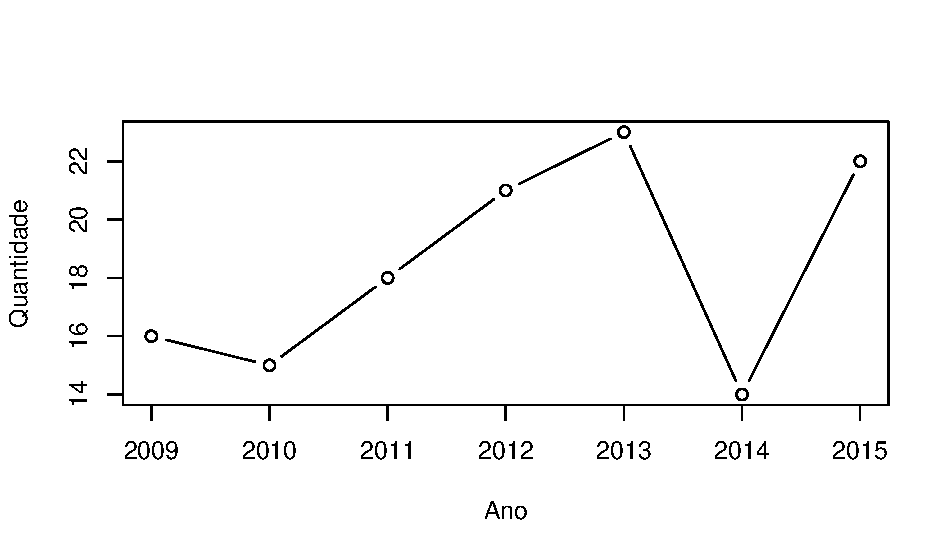
\includegraphics[width=1\textwidth]{./imagens/im_tools.pdf}
    \caption{Quantidade de soluções submetidas ao OAEI}
        \footnotesize{Fonte: \cite{cheatham2015results}.}
        \label{fig:oaei_imtools}
\end{figure}

Porém, de acordo com \citeonline{homoceanu2014putting}, apesar dos bons resultados apresentados, as soluções não estão prontas para alinhar dados automaticamente de forma confiável. Para isso, foi realizado um experimento equivalente ao executado pela OAEI. Entretanto, utilizando dados reais, que foram obtidos de 5 fontes diferentes (Freebase\footnote{\url{http://www.freebase.com/}}, DBPedia\footnote{\url{http://dbpedia.org}} , LinkedMDB\footnote{\url{http://www.linkedmdb.org}}, DrugBase\footnote{\url{http://www.drugbase.de/de/}} e NewYork Times\footnote{\url{http://www.nytimes.com}}). Além disso, o experimento permitiu notar que as características do modelo não eram considerados durante o processo de correspondência de instâncias.
        
Dentre as propriedades com suporte inadequado,  destaca-se a propriedade owl:sameAs, que é responsável por identificar recursos equivalentes. Além disso, essa se trata de uma propriedade transitiva. Dessa forma, se existem dois recursos equivalentes R1 e R2 e existe um terceiro recurso R3 que é equivalente a R2, então R1 é equivalente a R3. Como representado na Figura \ref{sameAs}.Tais características fazem com que a propriedade owl:sameAs seja uma das  mais utilizadas para alinhar dados na Web. Dessa forma, utilizar ferramentas que levem em consideração as características das propriedades é de grande importância para alinhar dados de forma confiável.
\begin{figure}[h]
\centering
\begin{tikzpicture}[node distance=1cm, auto,]
 %nodes
 \node[ellipse,draw] (r3) {R3};
 
 \node[above=of r3] (dummy) {};
 \node[right= of dummy,ellipse,draw](r2) {R2}
        edge[pil,<->, bend left=45] node[auto] {owl:sameAs} (r3);
 
 \node[left= of dummy,ellipse,draw] (r1) {R1}
        edge[dashed,<->, bend right=45] node[auto] {owl:sameAs} (r3)
        edge[pil,<->, bend left=45] node[auto] {owl:sameAs} (r2);
\end{tikzpicture}
\caption{Transitividade da propriedade owl:sameAs}
\label{sameAs}
\end{figure}

Neste contexto, este trabalho propõe uma abordagem independente de contexto para o alinhamento de dados conectados por meio de um processo de alinhamento que leva em consideração aspectos dos dados e  características do modelo ontológico. Assim, os recursos/instâncias analisados, além de alinhados através das propriedades de dados, podem ser alinhados través seus relacionamentos. Ademais, a proposta trata o problema do alinhamento entre datasets reais, permitindo que seja possível alinhar datasets distribuídos na Web de forma confiável.

\section{Objetivo}

Essa abordagem visa disponibilizar um mecanismo útil que permita alinhar semiautomaticamente recursos entre datasets diferentes. Além disso, a proposta também pretende facilitar a identificação e alinhamento de recursos duplicados dentro do mesmo dataset.
Dessa forma, o trabalho lida com aspectos mais gerais, como facilitar o alinhamento de dados, quanto com problemas específicos, como a definição de métricas para a análise de similaridade entre recursos, que sejam capazes de suportar os problemas provenientes dos datasets reais. Apesar de ser um trabalho com enfoque em engenharia de software, as suas contribuições estão mais voltadas para a área de Dados Conectados. Segue algumas dessas contribuições:

\begin{itemize}
        \item Construção de um processo para alinhar dados conectados independente de contexto;
        \item Definição de uma função de similaridade que contempla problemas provenientes de datasets reais (acentuação, ausência de propriedades, formatação e outros);
\end{itemize}

\section{Estrutura do trabalho}

Esta dissertação está dividida em 7 capítulos. O Capítulo 1 introduz a problemática e os objetivos do trabalho proposto, enaltecendo a necessidade de uma abordagem capaz de alinhar dados conectados. No Capítulo 2, são apresentados os conceitos relacionados ao tema deste trabalho, como RDF, Ontologias, Dados Conectados, Algoritmos de similaridade e Alinhamento de Dados Conectados.

No Capítulo 3, são apresentados os trabalhos relacionados à abordagem proposta. Algumas abordagens de alinhamento são descritas bem como comparadas com a solução proposta. Na conclusão do capítulo é apresentada uma tabela comparativa entre a abordagem proposta e os trabalhos relacionados apresentados.

O Capítulo 4 mostra como a proposta foi desenvolvida, tanto no processo de alinhamento por intermédio de um diagrama de atividades como na arquitetura através de um diagrama de componentes. Neste capítulo, todas as etapas do processo bem como os componentes da arquitetura são descritos detalhadamente.

No Capítulo 5 é apresentado um estudo de caso. Nele é descrita a plataforma QIE, um sistema que cruza dados da Revista Brasileira de Informática na Educação (RBIE), Simpósio Brasileiro de Informática na Educação (SBIE) e Workshop de informática na Escola (WIE) com dados extraídos da plataforma LATTES. Além disso, é descrito como o processo foi utilizado para alinhar os dados dos pesquisadores e de suas produções científicas entre essas bases.

No Capítulo 6, um experimento foi projetado para avaliar, em termos de eficácia através das métricas de precisão, revocação e medida-f, a abordagem proposta, em comparação com RiMOM \cite{zhang2015rimom} , Lily \cite{wang2015lily} e LogMap \cite{jimenez2015logmap}. Cada conjunto de alinhamento gerado é avaliado e uma discussão geral é apresentada ao final do capítulo.

Por fim, no Capítulo 7, são apresentadas as considerações finais deste trabalho. bem como são definidos alguns trabalhos futuros.


% ----------------------------------------------------------
% ELEMENTOS PÓS-TEXTUAIS (Referências, Glossário, Apêndices)
% ----------------------------------------------------------
\postextual

\bibliography{bibliografia}

\end{document}
